\section{Caso de Teste 2}
\label{sec:cenario2}

Este caso de teste está dividido em 5 (cinco) cenários, os quais são apresentados a seguir, contemplando todo o processo de auto-localização
em cada exemplo, a partir da apresentação das imagens a seguir, Figura \ref{img:cen2_ex1} a Figura \ref{img:real_cen2_ex5}.

\subsection{Cenário 1}

Cenário utilizando velocidade de rotação em 10 graus por segundo:

{\centering
\includegraphics[scale=0.4]{figuras/cen2_ex1.eps}
\captionof{figure}{Caso de Teste 2 - Cenário 1}
\label{img:cen2_ex1}
\par}

{\centering
\includegraphics[scale=0.2]{figuras/real_cen2_ex1.eps}
\captionof{figure}{Posição Real do Caso de Teste 2 - Cenário 1.}
\label{img:real_cen2_ex1}
\par}

\subsection{Cenário 2}

Cenário utilizando velocidade de rotação em 30 graus por segundo:

{\centering
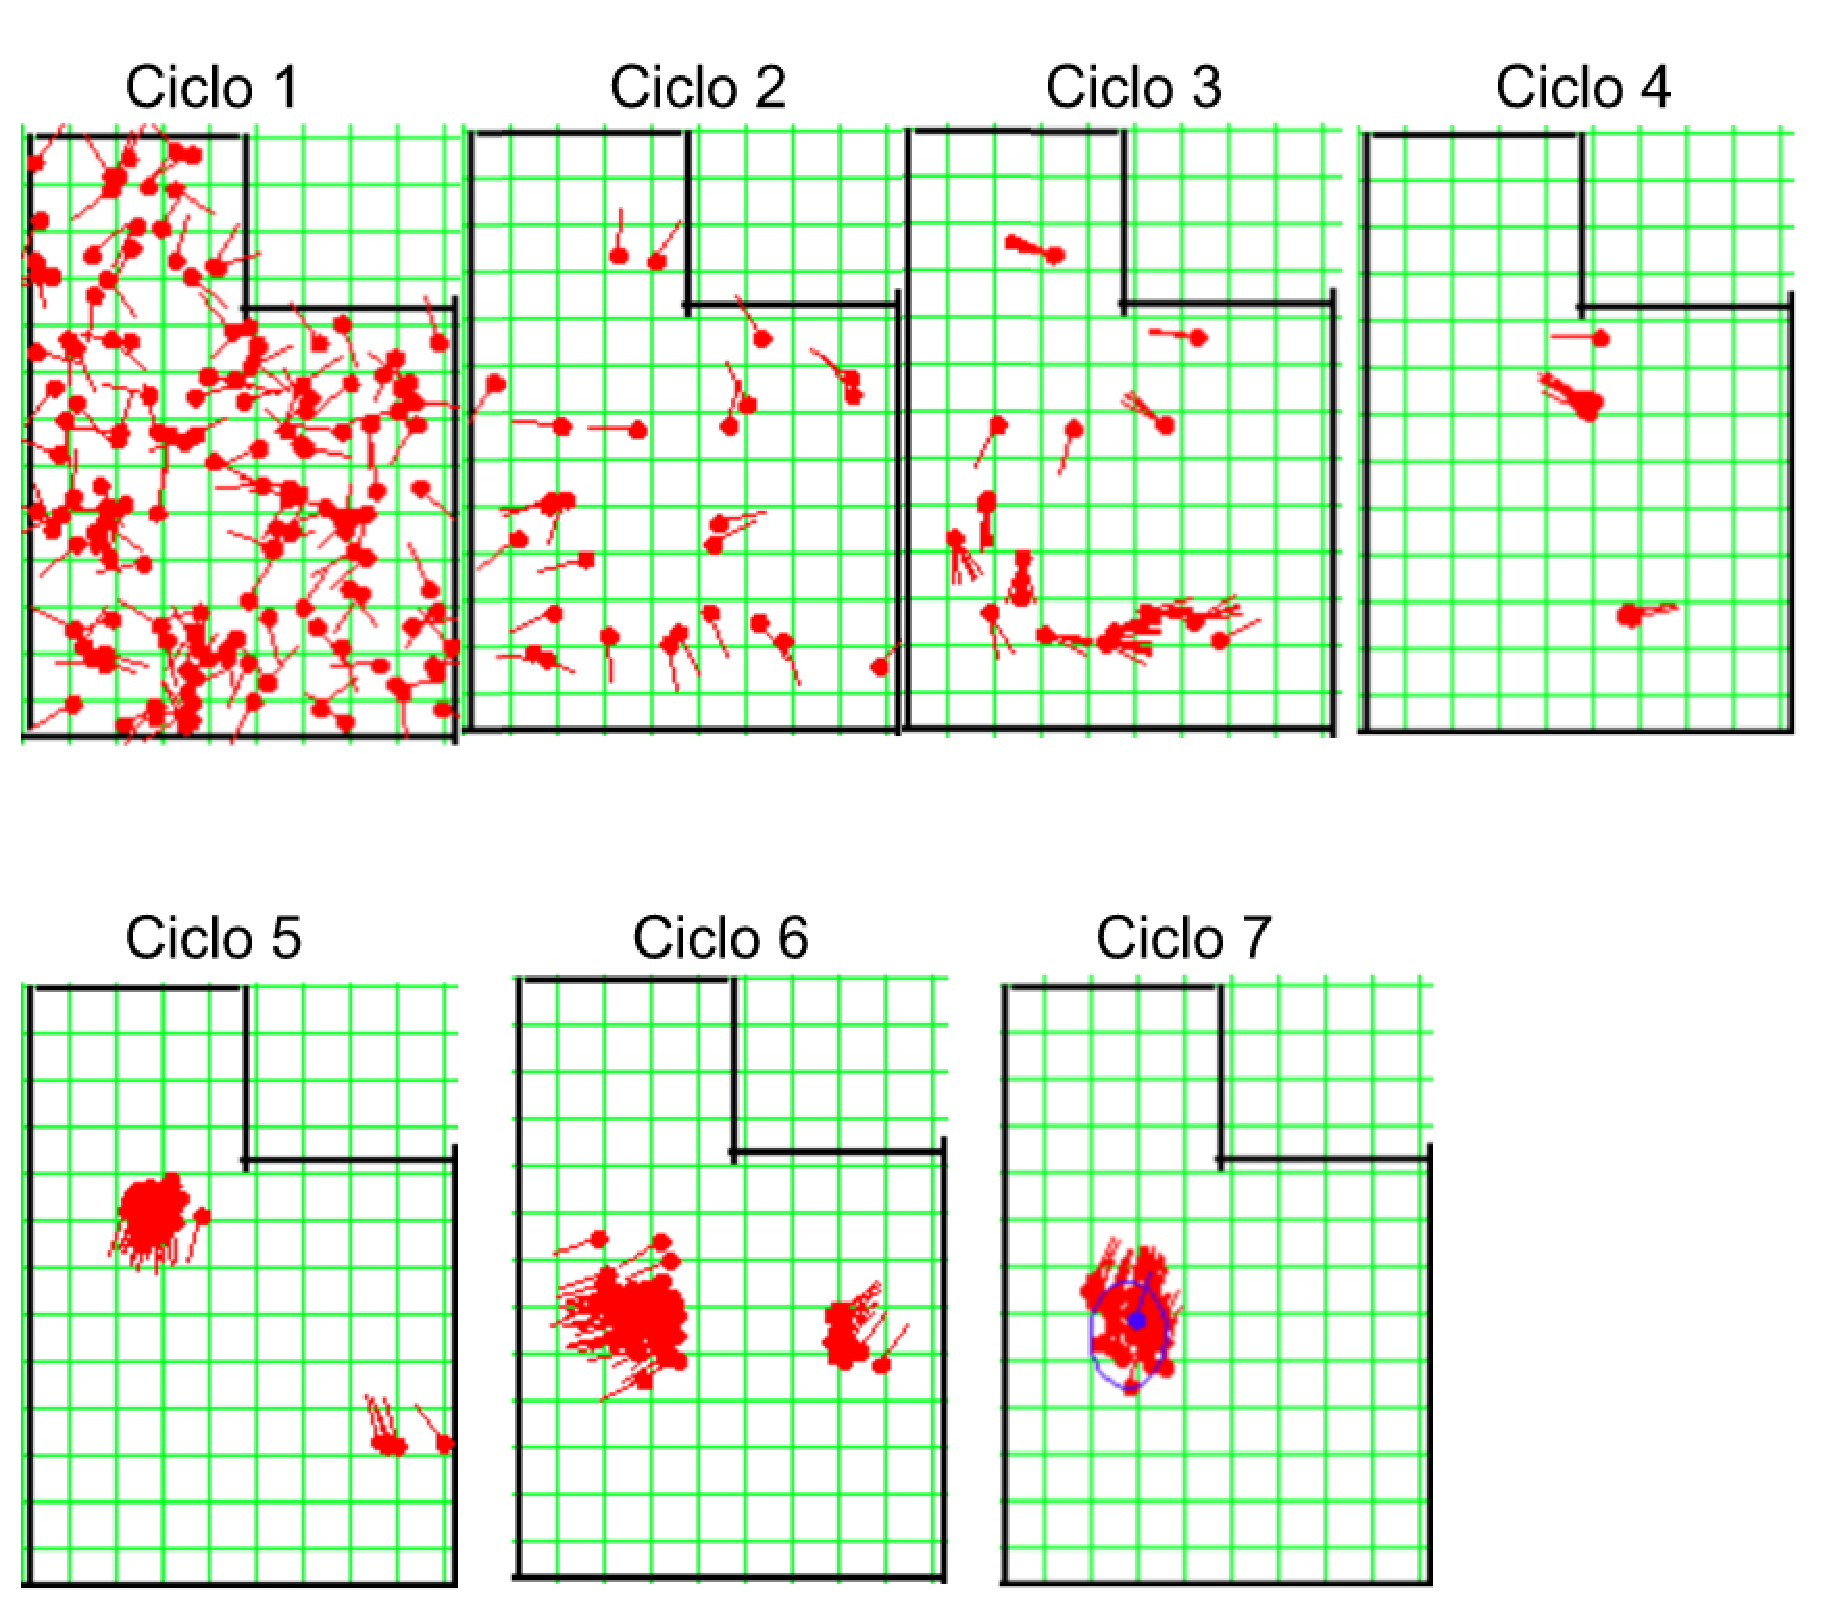
\includegraphics[scale=0.4]{figuras/cen2_ex2.eps}
\captionof{figure}{Caso de Teste 2 - Cenário 2}
\label{img:cen2_ex2}
\par}

{\centering
\includegraphics[scale=0.2]{figuras/real_cen2_ex2.eps}
\captionof{figure}{Posição Real do Caso de Teste 2 - Cenário 2.}
\label{img:real_cen2_ex2}
\par}

\subsection{Cenário 3}

Cenário utilizando velocidade de rotação em 50 graus por segundo:

{\centering
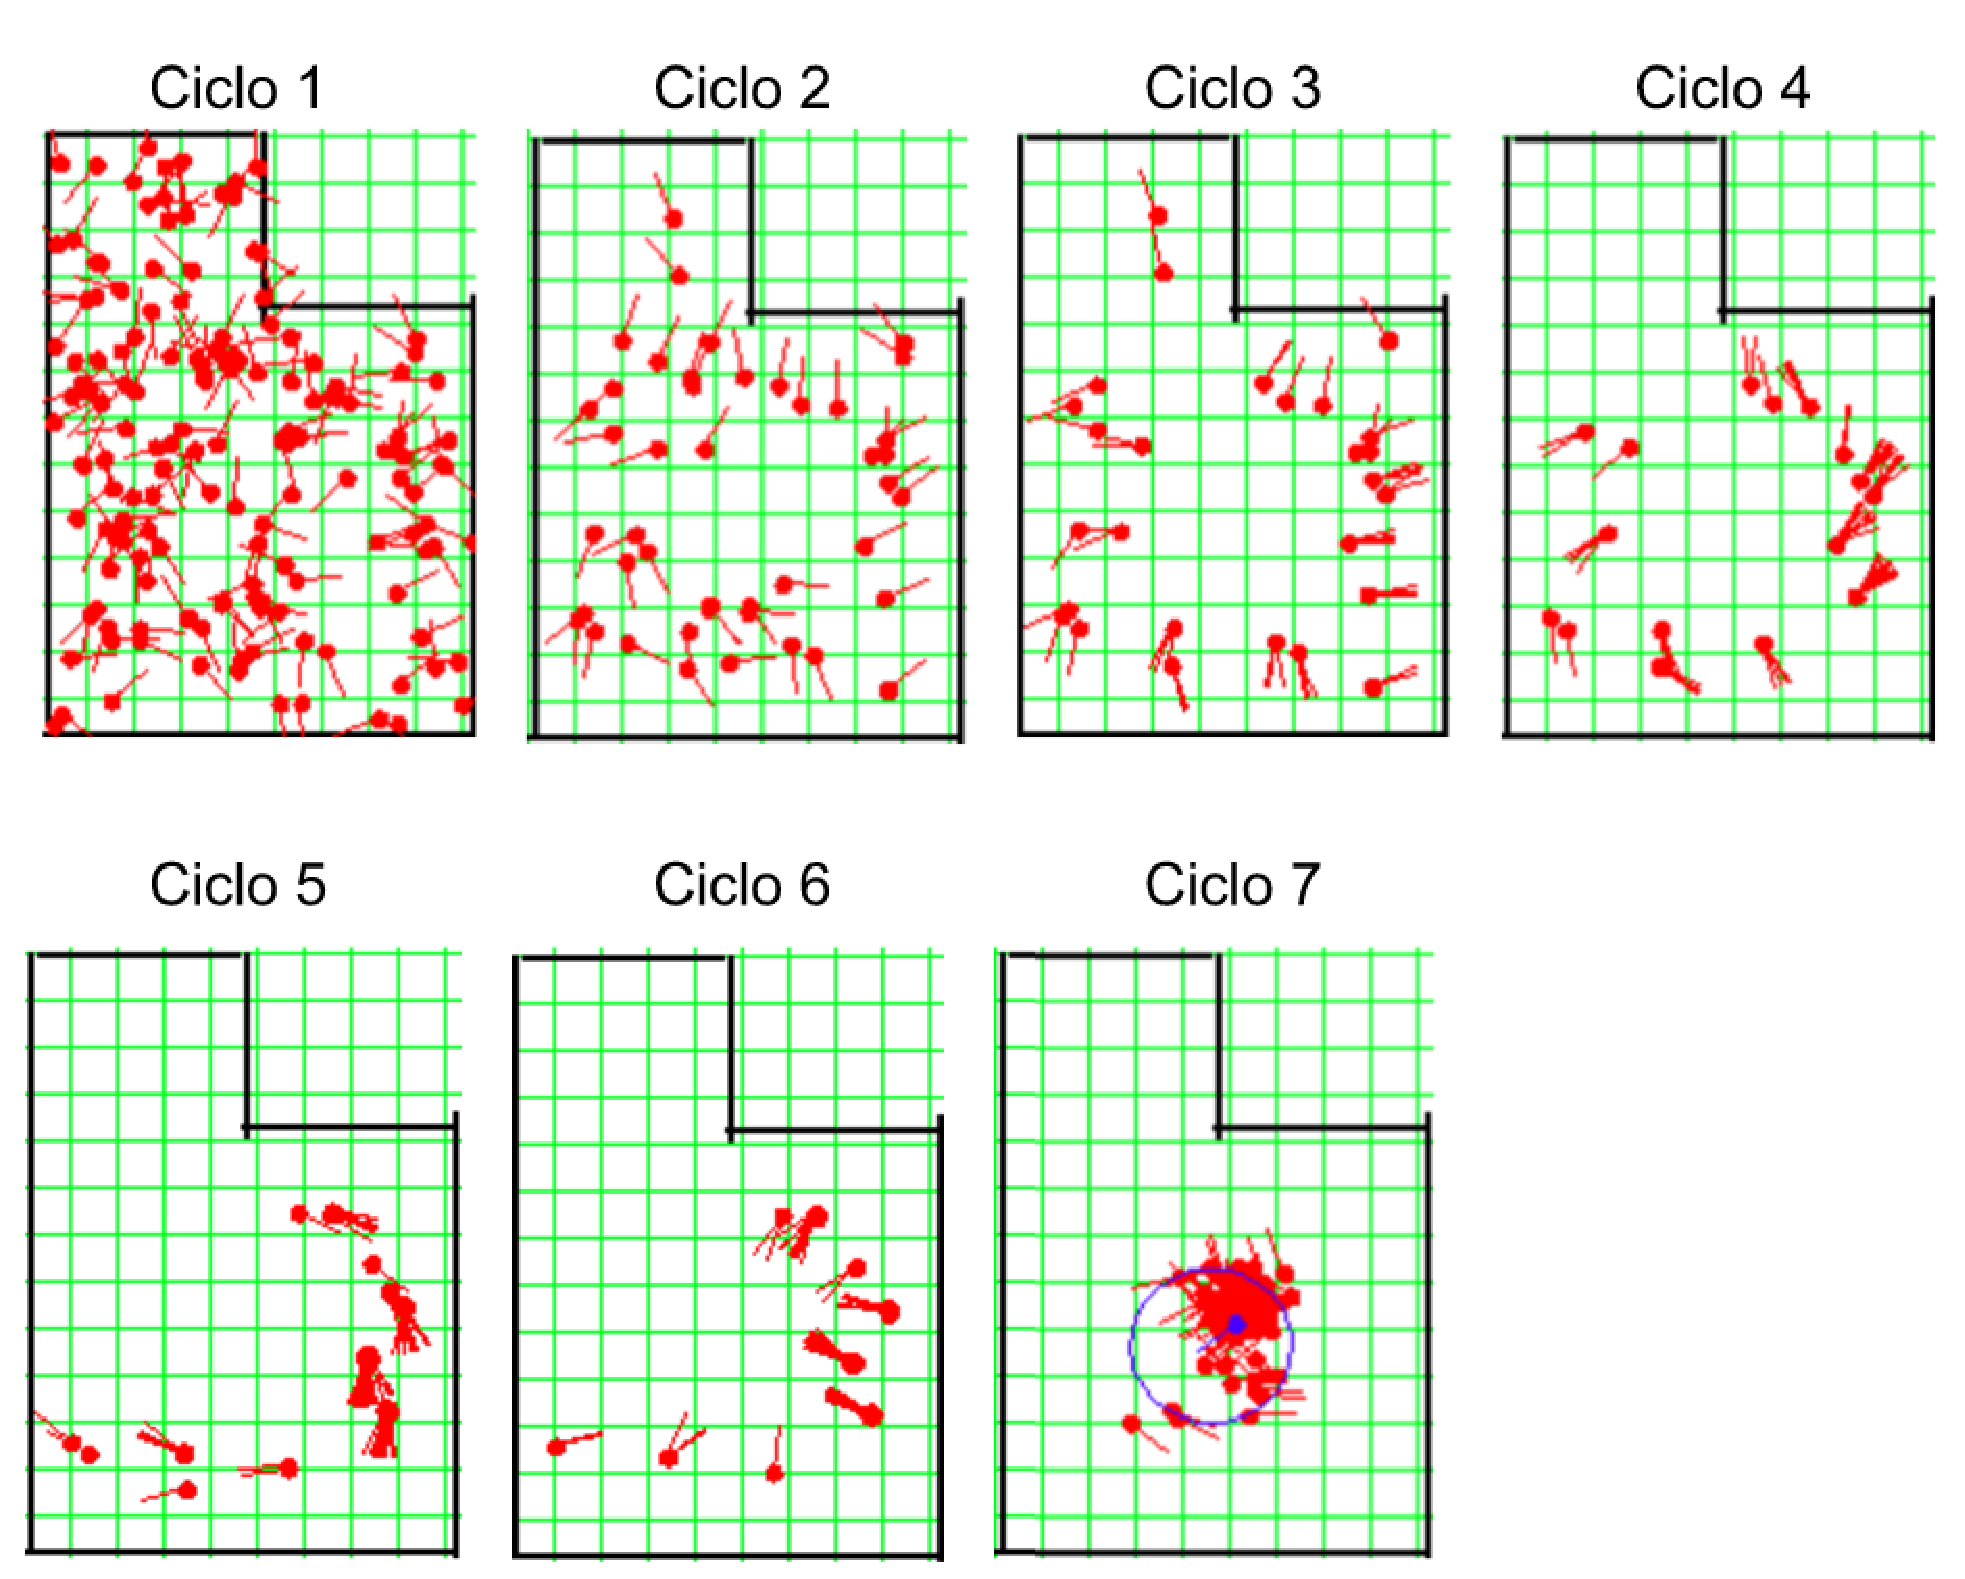
\includegraphics[scale=0.4]{figuras/cen2_ex3.eps}
\captionof{figure}{Caso de Teste 2 - Cenário 3}
\label{img:cen2_ex3}
\par}

{\centering
\includegraphics[scale=0.2]{figuras/real_cen2_ex3.eps}
\captionof{figure}{Posição Real do Caso de Teste 2 - Cenário 3.}
\label{img:real_cen2_ex3}
\par}

\subsection{Cenário 4}

Cenário utilizando velocidade de rotação em 70 graus por segundo:

{\centering
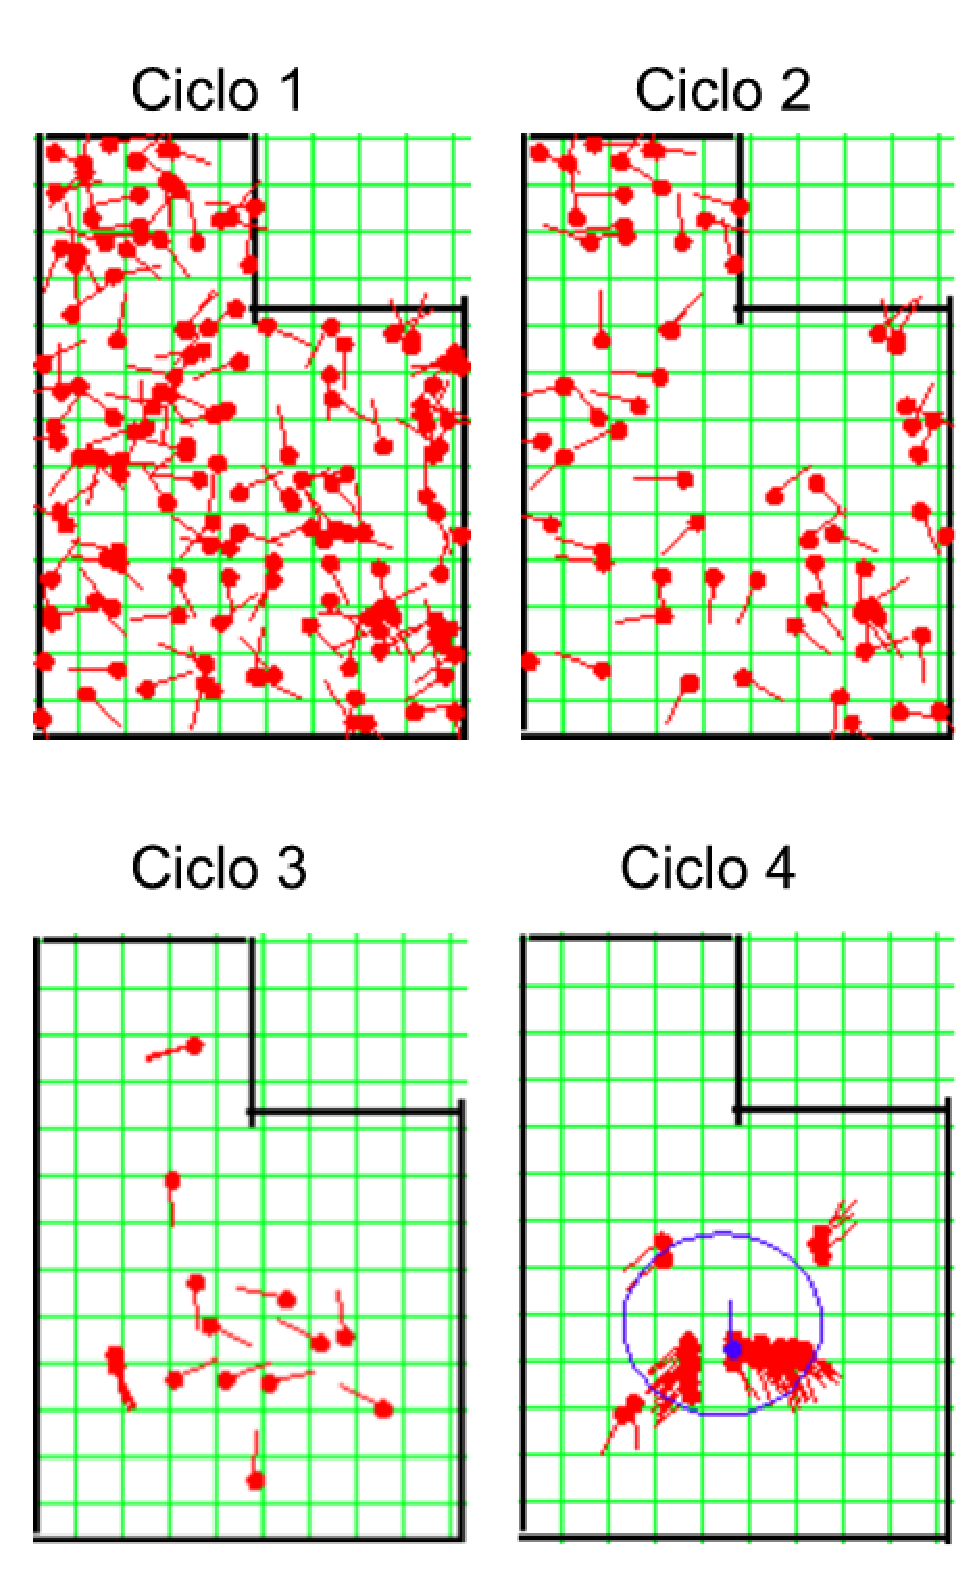
\includegraphics[scale=0.4]{figuras/cen2_ex4.eps}
\captionof{figure}{Caso de Teste 2 - Cenário 4}
\label{img:cen2_ex4}
\par}

{\centering
\includegraphics[scale=0.2]{figuras/real_cen2_ex4.eps}
\captionof{figure}{Posição Real do Caso de Teste 2 - Cenário 4.}
\label{img:real_cen2_ex4}
\par}

\subsection{Cenário 5}

Cenário utilizando velocidade de rotação em 90 graus por segundo:

{\centering
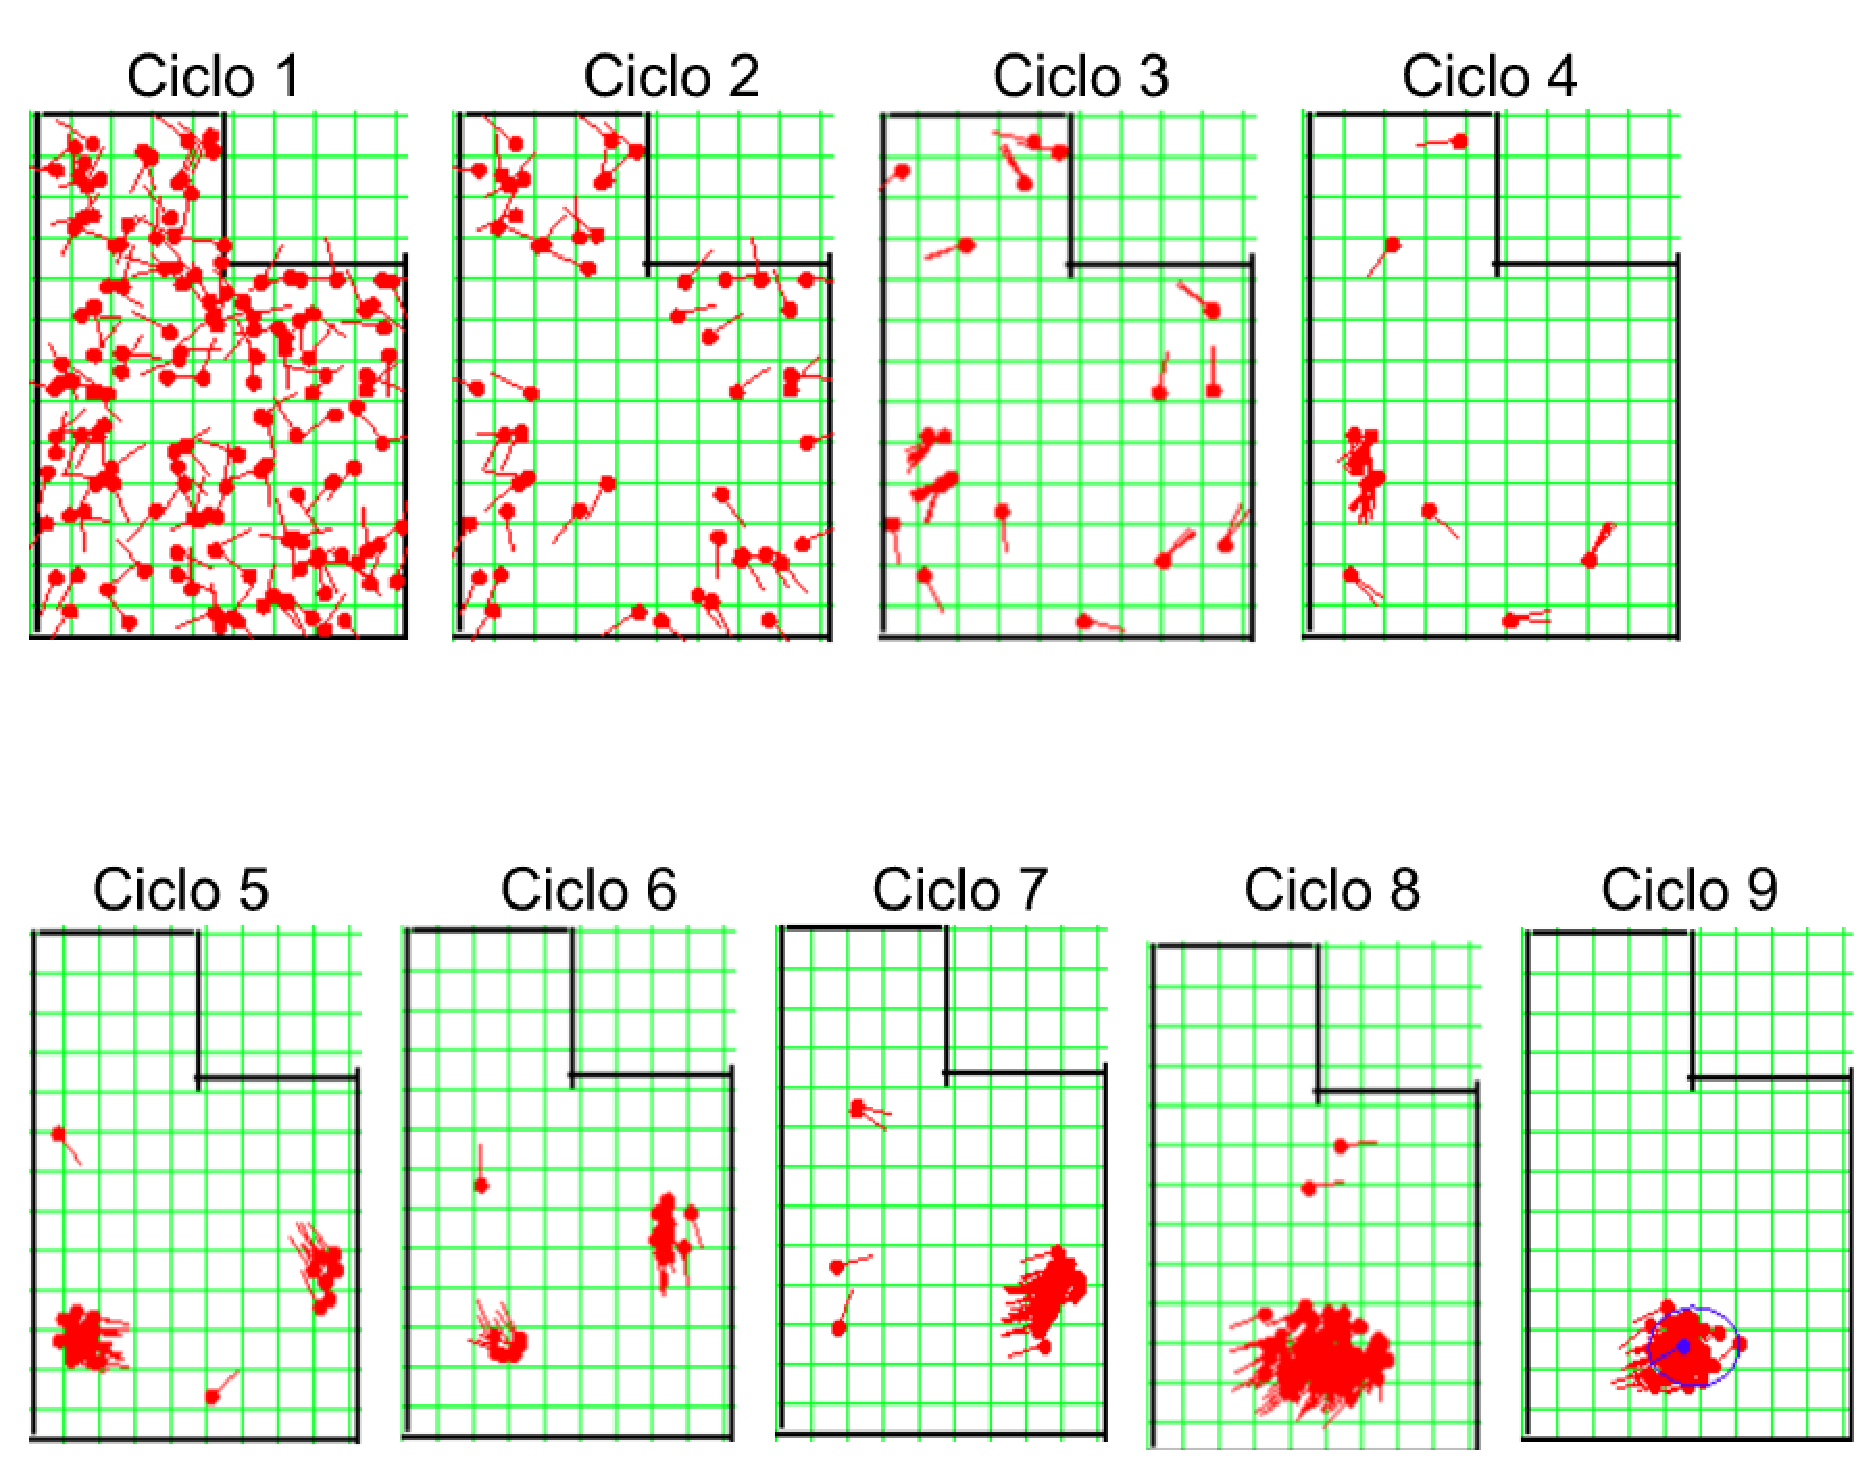
\includegraphics[scale=0.4]{figuras/cen2_ex5.eps}
\captionof{figure}{Caso de Teste 2 - Cenário 5}
\label{img:cen2_ex5}
\par}

{\centering
\includegraphics[scale=0.2]{figuras/real_cen2_ex5.eps}
\captionof{figure}{Posição Real do Caso de Teste 2 - Cenário 5.}
\label{img:real_cen2_ex5}
\par}
